\documentclass{foi}
\usepackage[utf8]{inputenc}
\usepackage{lipsum}

\vrstaRada{\projekt} % \diplomski \projekt \seminar \zavrsni
\title{Kamen, Škare, Papir}

\author{Josip Petanjek}
\spolStudenta{\musko} % \zensko ili \musko
\mentor{Markus Schatten}
\spolMentora{\musko} % \zensko ili \musko
\godina{2020}
\mjesec{prosinac}
\date{2020}
%\status{redoviti}
\indeks{0016124756}
\smjer{Informacijsko i programsko inženjerstvo} % (ili Poslovni sustavi, Ekonomika poduzetništva, Primjena informacijske tehnologije u poslovanju, Informacijsko i programsko inženjerstvo, Baze podataka i baze znanja, Organizacija poslovnih sustava, Informatika u obrazovanju)
\titulaProfesora{Dr. sc.}

\sazetak{Kamen, škare, papir je društvena igra između dva igrača. Igra se igra na principu da oba igrača istovremeno daju jedan od tri moguća pokreta (stanja), te se s obzirom na pokret odabire pobjednik. Projektni zadatak se realizira na principu izgradnje nekoliko agenata baziranih na istom sučelju koji igraju igru u turniru, ali svaki sa svojim specifičnim ponašanjima, koja naposljetku daju odabrani pokret (kamen, škare ili papir).
Neka od ponašanja agenata mogu biti CopyCat, Gubitnik, Igrac, ProtuCopyCat, UvijekKamen, UvijekŠkare, UvijekPapir.
Na početku se inicijalizira veličina turnira, odnosno koliko agenata se želi stvoriti, te se nasumično stvaraju tipovi agenata uz jednog agenta koji predstavlja igrača. U turniru se onda uparuju agenti, te se izvodi njihovo ponašanje, s obzirom na odabrane pokrete, turnir odlučuje pobjednika, te gubitnika eliminira iz turnira, ovo ponašanje se nastavlja dok god se ne dođe do pobjednika.
}

\kljucneRijeci{Kamen, Škare, Papir, Agent, CopyCat, CounterCopyCat, Turnir.}

\begin{document}

\maketitle

\tableofcontents

\pagestyle{plain}
\chapter{Uvod}

Igre gestama velika su obitelj igara koje su neovisno otkrivene u raznim točkama povijesti, čiji je kamen, škare, papir međunarodno najuspješniji primjer. To je igra japanskog podrijetla, poznat kao "jaken", čiji je izvor igra zvana "mushi-ken" koji se igrao sa žabom, zmijom i pužem \cite{towardsAI2020}.

Njezine strategije se mogu podjeliti na tri djela:
\begin{itemize}
    \item Temeljne strategije
    \item Rubne strategije
    \item Meta strategije
\end{itemize}
Ovaj rad baviti će se temeljnim strategijama, odnosno stvaranjem agenata koji će njih oponašati.
Cilj je emulirati prave igrače i njihove strategije te ponašanja.

Na ovo će se nadodati i sustav, odnosno agent, za provođenje turnira koji zapravo omogućava interakciju između agenata, te agent za igranje od strane korisnika programa.


Sam projekt realizirati će se u Java programskom jeziku.

\chapter{Korištena tehnologija}
Za izradu ovog projektnog zadatka korišten je operacijski sustav Microsoft Windows,točnije Microsoft Windows 10 Educational edition.
Za izradu dokumentacije projekta korišten je LaTeX. Za pisanje korišten je Overleaf - on-line LaTeX alat čija je svrha kreiranje LaTeX dokumenata na internetu. 

Koristi se razvojno okruženje Apache NetBeans IDE 11.2, te jezik Java JDK 13 uz Maven tip projekta.

Jezik je odabran zbog jednostavnosti projekta, te zato što nema potrebe za kompleksnim ponašanjima.

Turnir agent koristi cikličko ponašanje, odnosno ponavljanje iste radnje u ciklusima.


\chapter{Razrada teme}

Višeagentski sustavi su sustavi u kojima postoji nekoliko neovisnih agenata radeći u suradnji ili jedni protiv drugih kako bi zadovoljili cilj. Stvarni svijet
primjeri višeagentski sustava uključuju jata ptica i rojeve insekata \cite{RPS2006}. 

Ti agenti mijenjaju svoje ponašanje na temelju podataka koje prikupljaju iz okoline i od drugih agenata, odnosno, u našem primjeru, daje im se njihov prethodni pokret.
Ponašanja, ili strategije, proučiti ćemo u sljedećem poglavlju, te naposljetku i njihovu implementaciju.

\section{Općenito o kamen, škare, papir}

Kamen, škare, papir pripada grupi igara zvanim igre gestama, te je vrlo poznata divljem svijeta. To je iznimno jednostavna igra sa malo pravila ali puno implikacija, te je dobra podloga za više-agentne sustave.

Sastoji se od nekoliko jednostavnih pravila igre:
\begin{itemize}
    \item Kamen pobjeđuje Škare
    \item Škare pobjeđuju Papir
    \item Papir pobjeđuje Kamen
    \item Ako je pokret isti dolazi do neriješenog rezultata
    \item Pokret nije poznat prije igranja, odnosno oba igrača bacaju pokret u isto vrijeme
\end{itemize}

Jedan od ključnih principa igre je njezina nepredvidljivost \cite{towardsAI2020}, jer igra ima ograničen set poteza. 
Ako uopće nema vremenskog ograničenja, igrači imaju vremena da smisle  slučajnu vrijednost na kojoj će temeljiti svoju igru, ili da prevladaju vlastito i protivničko bacanje dok rezultat ne bude toliko zamršen mogao bi biti i slučajan. Obje ove mogućnosti imaju isti ishod - slučajna igra i jednaka očekivanja pobjeda tijekom vremena za bilo kojeg igrača.
Ako se igra brzo i u ritmu, igrači nemaju vremena niti pronaći izvor slučajnih poteza, niti previše razmisliti, ishod dakle određuje sposobnost igrača da brzo odabere strategiju, odbaci izgubljenu strategiju, ostane miran i analizira ponašanje svog protivnika.
Iz tog razloga, dok igra ima regionalne razlike, uvijek postoji brzo odbrojavanje ili skandiranje i brzo vrijeme obrade. 

Drugi ključni princip igre je njezin uravnoteženost\cite{towardsAI2020}, to je koncept da postoje tri sile koje se međusobno drže pod kontrolom. Ovaj koncept potječe iz Kine, ali se pojavljuje rano u japanskoj literaturi, povezan i s igrama i s raznovrsnim edukativnim filozofskim konceptima.

\subsection{Strategije}

Strategija ove igre je složena tema, općenito, strategiju možemo razdvojiti na tri područja \cite{towardsAI2020}:

\begin{itemize}
    \item Temeljne strategije - vrti se oko stvaranja brzih, gotovo automatskih ponašanja u kojima igrač, bez razmišljanja, prilagođava svoja bacanja protivniku na takav način da pobjeđuje više od polovice vremena.
    \item Rubne strategije - obuhvaća strategiju koja se odnosi na timsku igru, vrijeme i psihologiju.
    \item Meta strategije - Događaji izvan same igre, koji unatoč tome utječu na ishod.
\end{itemize}

Temeljne strategije koriste ozbiljni igrači, kako bi pobjedili, razmišljanja povezana sa ovim strategijama su:
\begin{itemize}
    \item Kao pobjednik zadnjeg bacanja: Igrajte isto bacanje kao i prošli put.
    \item Kao pobjednik zadnjeg bacanja: Igrajte bacanje kojim biste pobijedili posljednje bacanje.
    \item Kao pobjednik zadnjeg bacanja: Igrajte bacanje koje bi izgubilo do zadnjeg bacanja.
    \item Kao gubitnik zadnjeg bacanja: Kopirajte pobjedničko bacanje.
    \item Kao gubitnik zadnjeg bacanja: Igrajte bacanje koje bi pobijedilo pobjedničko bacanje.
    \item Kao gubitnik zadnjeg bacanja: Igrajte bacanje koje bi izgubilo pobjedničko bacanje.
\end{itemize}
    
Ovi "atomi", iliti opcije, se koriste u pravome svijetu, te će zato biti temelj za naše agente.

Postoji nekoliko širokih statističkih opažanja koja mogu pomoći u određivanju početne strategije:

Kamen čini oko 36\% bacanja, papir 34\%, a škare 30\%. Čini se da su ti omjeri istiniti u raznim vremenima, mjestima i vrstama igara.
Pobjednici posljednje bacanje ponavljaju daleko češće nego poraženi.
Ali samo dobar igrač može razviti strategiju u stvarnom vremenu i dosljedno pobjeđivati.

Rubne strategije se temelje na vremenskom tempiranju, te ne utječu na našu implementaciju ali u pravom svijetu imaju podosta utjecaja.

Što je brža igra to je vjerojatnije da će igrači igrati ‘zadane’ poteze (više bacanja kamena, više ponavljanja pobjedničkih bacanja), a manje sposobni postići pseudo-slučajnost. Brže igre pokazuju veću razliku u stopi pobjede među igračima.

Također je važna strogost pravila. Kad su pravila vrlo stroga, igrači u nizu poraza imaju malo mogućnosti. Kada su pravila manje čvrsta, igrač koji gubi može promijeniti ruku ili promijeniti vrijeme u nadi da će pobjediti.

Naposljetku, pravila bodovanja imaju snažan utjecaj,ova igra se obično igra u setovima "najbolje od tri", makar u ovom projektu će se igrati samo jedan set. Broj bacanja koje igrač mora napraviti prije nego što ostvari pobjedu ima statistički značajan utjecaj na pobjedu.

"Profesionalni" kamen, škare, papir -  često se igra kao brzi slijed od tri ili pet igara "najbolje od tri" bez prekida između njih - tako da ima dovoljno vremena za učenje protivničkog ponašanja.

Meta strategije neće imati pre veliki utjecaj na ovaj projekt, ali u stvarnom životu ima veliki utjecaj.

Noviji igrači su više nasumični od ozbiljnih igrača, pa ih je teže pobijediti, a također ih je teže pobijediti.
Sami igrači su ranjivi na tendenciju ka pogrešci uzrokovanoj nehotičnom percepcijom' nepravednosti u igri. Takvi igrači često će nepotrebno mijenjati bacanja ili ponavljati obrasce jer osjećaju da bi 'trebali' pobijediti.
Blefiranje i umne igre su veliki dio. Slijedi anegdota:
Vidio sam igrača kako se došetao do protivnika neposredno prije igre i rekao: "Planirate li ponovno izbaciti kamen? Super, čekat ću. " Kao i kod pokera, tolerancija na ovu vrstu tehnike varira od mjesta do mjesta događaja.

\subsection{Povijest}


Igre gestama velika su obitelj igara koje su neovisno otkrivene u raznim točkama povijesti, čiji je kamen, škare, papir međunarodno najuspješniji primjer. To je igra japanskog podrijetla, poznat kao "jaken", čiji je izvor igra zvana "mushi-ken" koji se igrao sa žabom, zmijom i pužem \cite{towardsAI2020}.

\begin{figure}[h!]
    \centering
    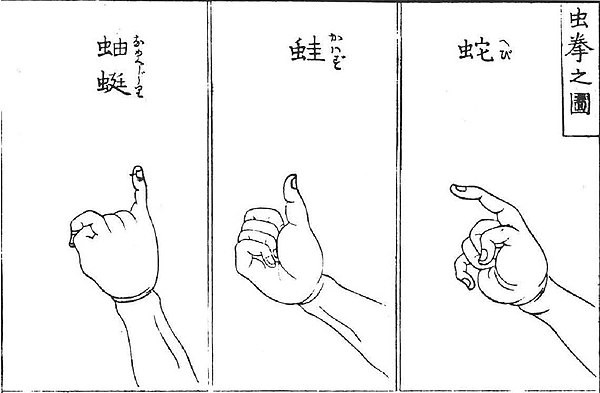
\includegraphics[width=0.9\textwidth]{slike/slika1.jpg}
    \caption{Mushi-ken geste (Izvor: \cite{towardsAI2020})}
\end{figure}

Poput mushi-ken, kamen, škare, papir je bio minimalna sansukumi igra sa samo tri mogućnosti. Ostale igre gesta sansukumi diljem Azije mogu imati pet ili čak četiri mogućnosti.

Igre gesta koje se ne temelje na sansukumiju često se temelje na neparnim / neparnim ishodima - uključujući vjerojatnosti i izjednačenja, ali i složenijim varijantama.

Od sredine 20. stoljeća, Janken se proširio svijetom izvan Japana, poprimajući mnoga imena i razvijajući vlastite inačice i skupove pravila. Tijekom 1980-ih Janken je shvaćen prilično ozbiljno, a u to su vrijeme postojale i značajne analize strategije u Kini i Japanu, te neki veliki turniri.

Nažalost, profil igre je pao tijekom posljednjih 20-ak godina; još uvijek postoje neke velike, ali ne postoji snažno upravno tijelo ni u Japanu ni globalno.

U 90-ima, kada se u nekim dijelovima Japana obično igrao za novac, igra "najbolje od tri" mogla bi biti gotova za četiri ili pet sekundi \cite{towardsAI2020}.

\section{Implementacija}

Ova implementacija bazirana je na agentima koji s obzirom na prijašnji pokret protivnika odabiru svoj pokret, odnosno provode strategiju.

Strategije su inspirirane prema knjižici za agente kamen, škare, papir \cite{agentcomparison}.

Agenti koji igraju igru se instanciraju u agentu turnir, koji ih tada spariva u parove te poziva njihovo ponašanje, nadalje eliminira se gubitnik, sve dok ne ostane samo jedan agent, te se on proglašava pobjednikom.

Sam turnir pokreće se u glavnoj klasi, te je potrebno zadati broj agenata u turniru.

\begin{figure}[h!]
    \centering
    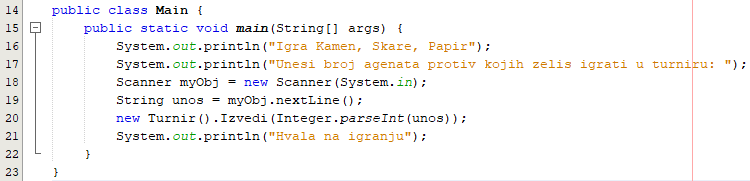
\includegraphics[width=0.9\textwidth]{slike/Screenshot_3.png}
    \caption{Klasa Main, vlastita izrada}
\end{figure}

Također, postoji i agent za igrača, koji traži od korisnika da unese odabrani pokret.

Tijekom igre ispisuje se tip agenta, te svaki njegov odabrani pokret.

Slijedi detaljno objašnjenje implementacija klasa.

\clearpage

\subsection{Abstraktna klasa Pokret i  klase Kamen, Skare, Papir}

Abstraktna klasa Pokret sama za sebe naravno nema nikakvu funkciju, samo nam služi kao indikator za klase koje će ju proširiti, dakle klase kamen, škare i papir.

\begin{figure}[h!]
    \centering
    
\includegraphics[width=0.9\textwidth]{slike/Screenshot_1.png}
    \caption{Klasa Pokret, vlastita izrada}
\end{figure}

Klase ovog tipa koristiti će se kao rezultat za ponašanje pojedinih agenata i njihovih implementacija.

U svakoj klasi potrebno je samo implementirati funkciju "toString" radi boljeg ispisa.

\begin{figure}[h!]
    \centering
    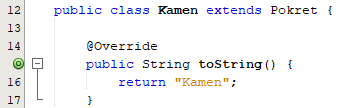
\includegraphics[width=0.5\textwidth]{slike/Screenshot_11.png}
    \caption{Klasa Kamen, vlastita izrada}
\end{figure}

\begin{figure}[h!]
    \centering
    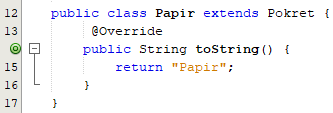
\includegraphics[width=0.5\textwidth]{slike/Screenshot_12.png}
    \caption{Klasa Škare, vlastita izrada}
\end{figure}

\begin{figure}[h!]
    \centering
    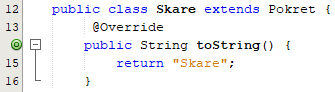
\includegraphics[width=0.5\textwidth]{slike/Screenshot_13.png}
    \caption{Klasa Papir, vlastita izrada}
\end{figure}

\clearpage
\subsection{Sučelje Agent}

Sučelje Agent koristimo za implementaciju različitih ponašanja i strategija agenata, koristi se da bi mogli u turnir primiti klase sa istim operacijama.

\begin{figure}[h!]
    \centering
    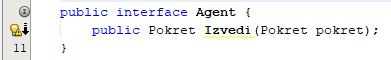
\includegraphics[width=0.9\textwidth]{slike/Screenshot_2.png}
    \caption{Klasa Agent, vlastita izrada}
\end{figure}

U ovom slučaju to je operacija "Izvedi", koja nam vraća objekt tipa "Pokret" te prima isti, odnosno daje se pokret protivnika u prošloj rundi, a vraća se pokret ovisno o strategiji određenog agenta.

\clearpage

\subsection{Agent Copy Cat}

Klasa Agent Copy Cat je implementacija abstraktne klase Agent, te je zato potrebno implementirati funkciju izvedi.

\begin{figure}[h!]
    \centering
    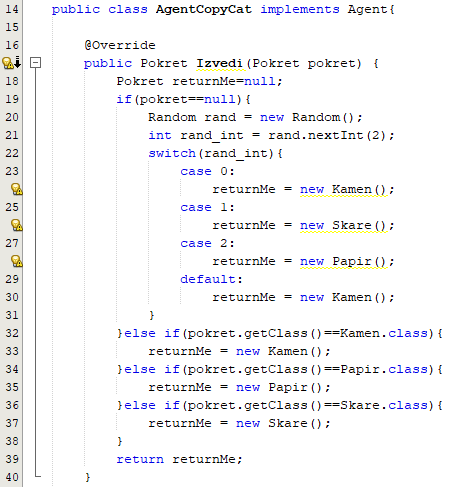
\includegraphics[scale=0.9]{slike/Screenshot_4.png}
    \caption{Klasa AgentCopyCat, vlastita izrada}
\end{figure}

Glavno ponašanje ovog agenta temelji se na zadnjem pokretu protivnika, kojeg mu turnir zadaje. Dakle, ovaj agent kopira zadnji pokret svojeg protivnika te daje to kao svoj pokret.

Ako nema prošlog pokreta protivnika, daje se nasumični pokret.

\clearpage

\subsection{Agent Gubitnik}

Klasa Agent Gubitnik je implementacija abstraktne klase Agent, te je zato potrebno implementirati funkciju izvedi.

\begin{figure}[h!]
    \centering
    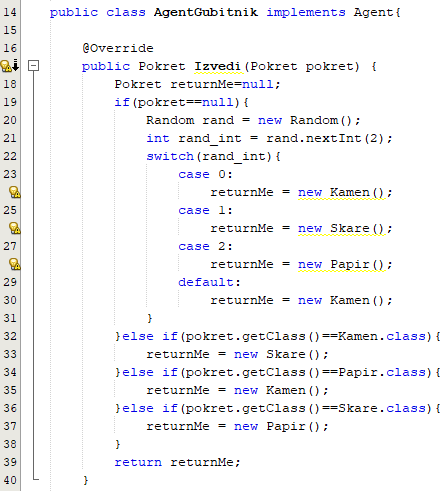
\includegraphics[scale=0.9]{slike/Screenshot_5.png}
    \caption{Klasa AgentGubitnik, vlastita izrada}
\end{figure}

Glavno ponašanje ovog agenta temelji se na zadnjem pokretu protivnika. Dakle, ovaj agent pokušava izgubiti turnir, te zato na temelju zadnjeg pokreta protivnika odabire onaj pokret koji bi mu izgubio igru.

Ako nema prošlog pokreta protivnika, daje se nasumični pokret.

\clearpage

\subsection{Agent Igrač}

Klasa Agent Igrač je implementacija abstraktne klase Agent, te je zato potrebno implementirati funkciju izvedi.

\begin{figure}[h!]
    \centering
    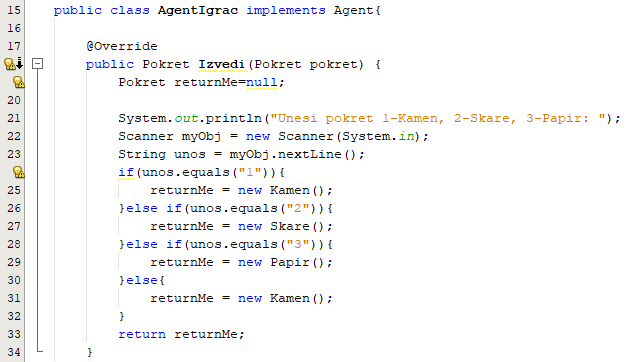
\includegraphics[scale=0.9]{slike/Screenshot_6.png}
    \caption{Klasa AgentIgrač, vlastita izrada}
\end{figure}

Glavno ponašanje ovog agenta temelji se na korisničkom unosu. Dakle ovisno o korisničkom unosu vraća se odabrani pokret.

\clearpage

\subsection{Agent Protu Copy Cat}
Klasa Agent Protu Copy Cat je implementacija abstraktne klase Agent, te je zato potrebno implementirati funkciju izvedi.
\begin{figure}[h!]
    \centering
    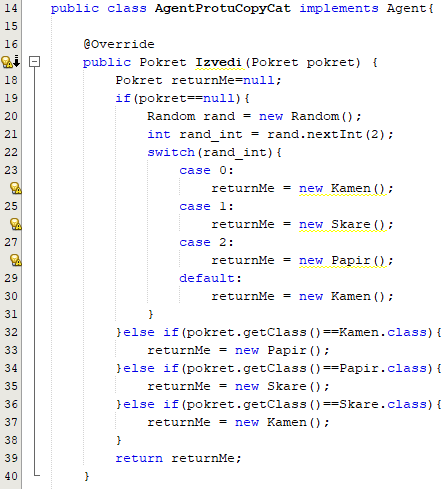
\includegraphics[scale=0.9]{slike/Screenshot_7.png}
    \caption{Klasa AgentProtuCopyCat, vlastita izrada}
\end{figure}

Glavno ponašanje ovog agenta temelji se na zadnjem pokretu protivnika. Dakle, ovaj agent pokušava pobjediti turnir, te zato na temelju zadnjeg pokreta protivnika odabire onaj pokret koji bi mu pobjedio igru.

Ako nema prošlog pokreta protivnika, daje se nasumični pokret.
\clearpage
\subsection{Agent Uvijek Kamen}
Klasa Agent Uvijek Kamen je implementacija abstraktne klase Agent, te je zato potrebno implementirati funkciju izvedi.
\begin{figure}[h!]
    \centering
    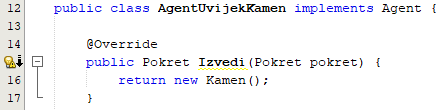
\includegraphics[scale=0.7]{slike/Screenshot_8.png}
    \caption{Klasa AgentUvijekKamen, vlastita izrada}
\end{figure}

Uvijek vraća pokret Kamen, bez obzira na prijašnji pokret protivnika.


\subsection{Agent Uvijek Škare}

Klasa Agent Uvijek Škare je implementacija abstraktne klase Agent, te je zato potrebno implementirati funkciju izvedi.

\begin{figure}[h!]
    \centering
    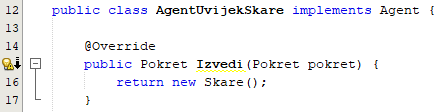
\includegraphics[scale=0.7]{slike/Screenshot_10.png}
    \caption{Klasa AgentUvijekŠkare, vlastita izrada}
\end{figure}

Uvijek vraća pokret Skare, bez obzira na prijašnji pokret protivnika.


\subsection{Agent Uvijek Papir}

Klasa Agent Uvijek Škare je implementacija abstraktne klase Agent, te je zato potrebno implementirati funkciju izvedi.

\begin{figure}[h!]
    \centering
    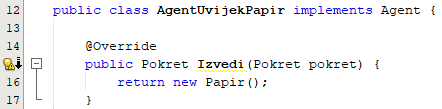
\includegraphics[scale=0.7]{slike/Screenshot_9.png}
    \caption{Klasa AgentUvijekPapir, vlastita izrada}
\end{figure}

On uvijek vraća pokret Papir, bez obzira na prijašnji pokret protivnika.

\clearpage

\subsection{Klasa Turnir}

Klasa turnir je agent koji zapravo upravlja interakcijama sa ostalim agentima, tako da ih uprauje i odlučuje o pobjedniku ovisno o njihovim pokretima.

Dakle iz izvorne klase dobiva broj agenata koji je potreban za turnir, te ih prema njemu generira nasumično, odnos nasumične klase, koje uz klasu igrača nadodaje u listu svih agenata.

Treba napomenuti da se sam broj agenata može smanjiti kako bi to bio paran broj, da se svi agenti mogu upariti.

\begin{figure}[h!]
    \centering
    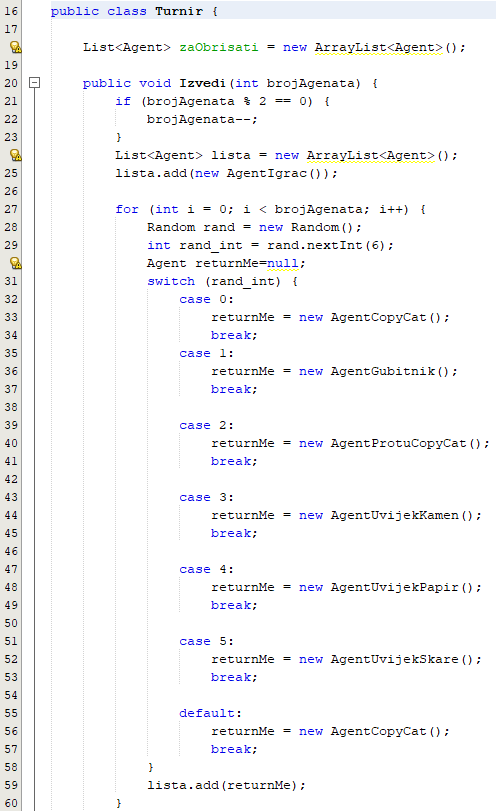
\includegraphics[width=0.5\textwidth]{slike/Screenshot_14.png}
    \caption{Klasa Turnir - generiranje agenata, vlastita izrada}
\end{figure}
\clearpage
Nadalje slijedi cikličko ponašanje, dakle svi agenti se uparuju u dva para, te se provodi funkcija "Odigraj" nad njima, što čini jednu rundu turnira, nakon jedne runde iz liste se brišu svi gubitnici, ovo se ponavlja dok ne ostane samo jedan agent u listi, odnosno pobjednik.

\begin{figure}[h!]
    \centering
    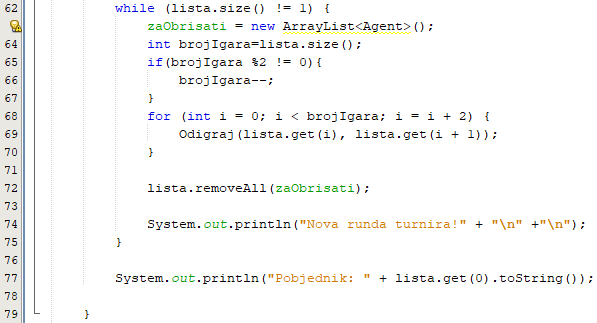
\includegraphics[width=0.85\textwidth]{slike/Screenshot_15.png}
    \caption{Klasa Turnir - runda turnira, vlastita izrada}
\end{figure}


\clearpage

Funkcija "Odigraj" je opet cikličko ponašanje koje ispituje oba agenta za njihov pokret dok ne pronađe pobjednika.

\begin{figure}[h!]
    \centering
    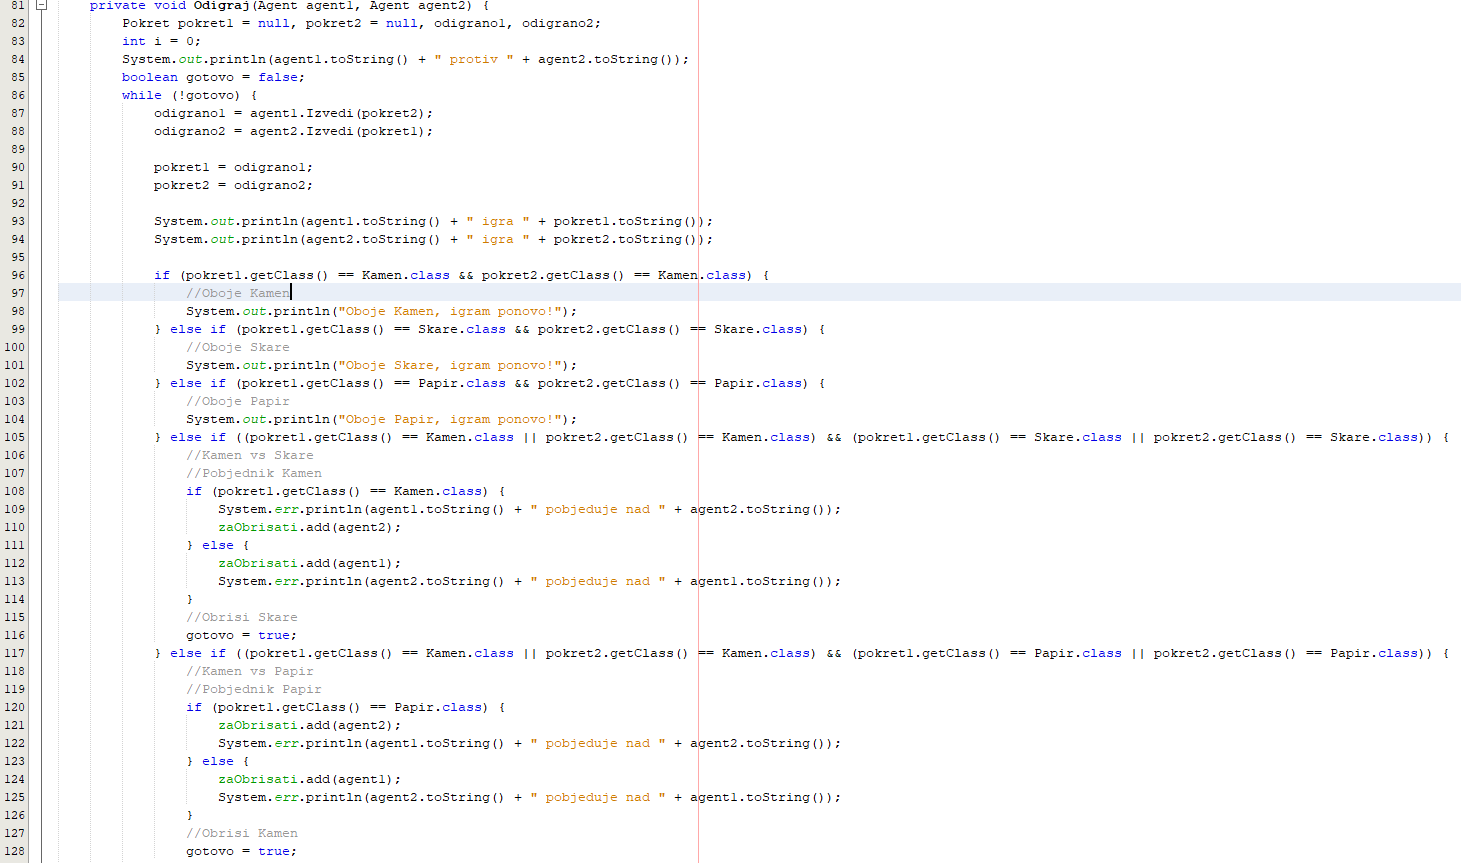
\includegraphics[width=0.85\textwidth]{slike/Screenshot_16.png}
    \caption{Klasa Turnir - funckija odigraj 1. dio, vlastita izrada}
\end{figure}

Ono ispisuje koji agenti trenutno igraju, te koji su njihovi pokreti.
Ispitivanje pokreta zapravo čini srž igre, dakle:

\begin{itemize}
    \item Ako je pokret isti dolazi do neriješenog rezultata - linija od 96 do 104 
    \item Kamen pobjeđuje Škare - linija od 105 do 116
    \item Škare pobjeđuju Papir - linija od 117 do 128
    \item Papir pobjeđuje Kamen - linija od 129 do 142
\end{itemize}

Također, imamo i ograničenje od 5 pokreta, odnosno, ako se dogodi da na primjer dva agenta uvijek škare zaigraju, neće doči do beskonačne petlje.

\begin{figure}[h!]
    \centering
    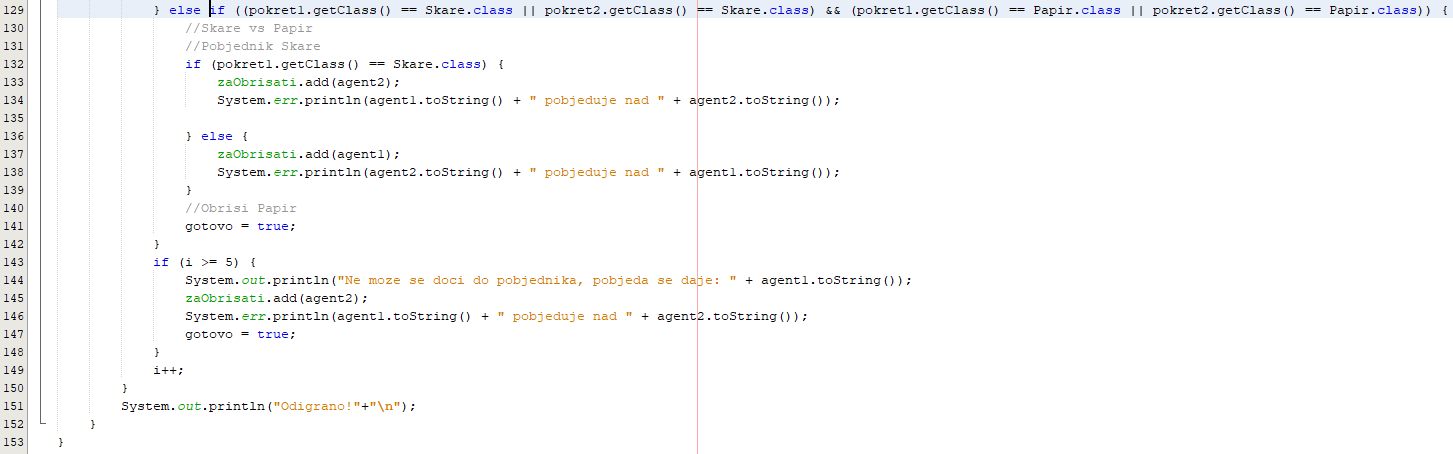
\includegraphics[width=0.85\textwidth]{slike/Screenshot_17.png}
    \caption{Klasa Turnir - funckija odigraj 2. dio, vlastita izrada}
\end{figure}
\clearpage

\subsection{Pokretanje}

Ako nije dostupni razvojni alat, moguće je pokrenuti program konzolno, prvo se je potrebno navigirati do mjesta gdje je kompiliran ".jar", te onda nad njim izvesti pokretanje, odnosno:
"java -jar VAS2020-1.jar"

\begin{figure}[h!]
    \centering
    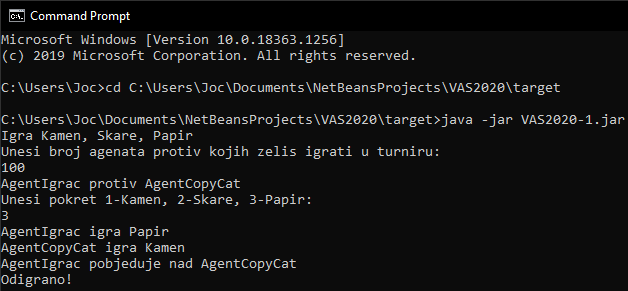
\includegraphics[width=0.85\textwidth]{slike/Screenshot_18.png}
    \caption{Primjer izvođenja, vlastita izrada}
\end{figure}

Naravno, nakon provođenja turnira, dolazimo do pobjednika, u ovom slučaju to je bio Agent Uvijek Papir.

\begin{figure}[h!]
    \centering
    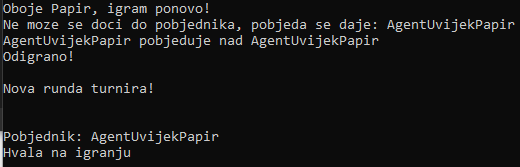
\includegraphics[width=0.85\textwidth]{slike/Screenshot_19.png}
    \caption{Pobjednik turnira, vlastita izrada}
\end{figure}


\chapter{Zaključak}

Igre gestama velika su obitelj igara koje su neovisno otkrivene u raznim točkama povijesti, čiji je kamen, škare, papir međunarodno najuspješniji primjer. Bilježe ju principi uravnoteženosti i predvidljivosti. To je vrlo klasična i jednostavna primjena za višeagentske sustave. Implementacija je vrlo jednostavna sa nekolicinom agenata sa svojim specifičnim strategijama, onim temeljnima, koje koriste i pravi igrači.

Osobno rad mi se je svidio, mislim da ima prostora za daljnju razradu, sa recimo strojnim učenjem agenata, te umreženom igrom, što je možda manjak naprema implementacijama sa nastave, koje to već imaju implementirano.

\printbibliography[title=Popis literature]
\addcontentsline{toc}{chapter}{Popis literature}

\listoffigures
\addcontentsline{toc}{chapter}{Popis slika}

\appendix
\renewcommand{\thechapter}{\arabic{chapter}}

\end{document}
